
% LaTeX Beamer file automatically generated from Doconce
% https://github.com/hplgit/doconce

%-------------------- begin beamer-specific preamble ----------------------

\documentclass{beamer}

\usetheme{red_shadow}
\usecolortheme{default}

% turn off the almost invisible, yet disturbing, navigation symbols:
\setbeamertemplate{navigation symbols}{}

% Examples on customization:
%\usecolortheme[named=RawSienna]{structure}
%\usetheme[height=7mm]{Rochester}
%\setbeamerfont{frametitle}{family=\rmfamily,shape=\itshape}
%\setbeamertemplate{items}[ball]
%\setbeamertemplate{blocks}[rounded][shadow=true]
%\useoutertheme{infolines}
%
%\usefonttheme{}
%\useinntertheme{}
%
%\setbeameroption{show notes}
%\setbeameroption{show notes on second screen=right}

% fine for B/W printing:
%\usecolortheme{seahorse}

\usepackage{pgf,pgfarrows,pgfnodes,pgfautomata,pgfheaps,pgfshade}
\usepackage{graphicx}
\usepackage{epsfig}
\usepackage{relsize}

\usepackage{fancyvrb}
\usepackage{minted} % requires pygments and latex -shell-escape filename
%\usepackage{anslistings}

\usepackage{amsmath,amssymb,bm}
%\usepackage[latin1]{inputenc}
\usepackage[utf8]{inputenc}
\usepackage{colortbl}
\usepackage[english]{babel}
\usepackage{tikz}
\usepackage{framed,anslistings}
% Use some nice templates
\beamertemplatetransparentcovereddynamic

% Delete this, if you do not want the table of contents to pop up at
% the beginning of each section:
\AtBeginSection[]
{
    \begin{frame}<beamer>[plain]
    \frametitle{}
    \tableofcontents[currentsection]
    \end{frame}
}

% Delete this, if you do not want the table of contents to pop up at
% the beginning of each section:
\AtBeginSection[]
{
    \begin{frame}<beamer>[plain]
    \frametitle{}
    \tableofcontents[currentsection]
    \end{frame}
}

% If you wish to uncover everything in a step-wise fashion, uncomment
% the following command:

%\beamerdefaultoverlayspecification{<+->}

\newcommand{\shortinlinecomment}[3]{\note{\textbf{#1}: #2}}
\newcommand{\longinlinecomment}[3]{\shortinlinecomment{#1}{#2}{#3}}

\newenvironment{notice_colors1admon}[1][]{\begin{block}{#1}}{\end{block}}
\newenvironment{notice_colors2admon}[1][]{\begin{block}{#1}}{\end{block}}
\newenvironment{notice_grayiconadmon}[1][]{\begin{block}{#1}}{\end{block}}
\newenvironment{notice_yellowiconadmon}[1][]{\begin{block}{#1}}{\end{block}}
\newenvironment{notice_mdfboxadmon}[1][]{\begin{block}{#1}}{\end{block}}
\newenvironment{summary_colors1admon}[1][]{\begin{block}{#1}}{\end{block}}
\newenvironment{summary_colors2admon}[1][]{\begin{block}{#1}}{\end{block}}
\newenvironment{summary_grayiconadmon}[1][]{\begin{block}{#1}}{\end{block}}
\newenvironment{summary_yellowiconadmon}[1][]{\begin{block}{#1}}{\end{block}}
\newenvironment{summary_mdfboxadmon}[1][]{\begin{block}{#1}}{\end{block}}
\newenvironment{warning_colors1admon}[1][]{\begin{block}{#1}}{\end{block}}
\newenvironment{warning_colors2admon}[1][]{\begin{block}{#1}}{\end{block}}
\newenvironment{warning_grayiconadmon}[1][]{\begin{block}{#1}}{\end{block}}
\newenvironment{warning_yellowiconadmon}[1][]{\begin{block}{#1}}{\end{block}}
\newenvironment{warning_mdfboxadmon}[1][]{\begin{block}{#1}}{\end{block}}
\newenvironment{question_colors1admon}[1][]{\begin{block}{#1}}{\end{block}}
\newenvironment{question_colors2admon}[1][]{\begin{block}{#1}}{\end{block}}
\newenvironment{question_grayiconadmon}[1][]{\begin{block}{#1}}{\end{block}}
\newenvironment{question_yellowiconadmon}[1][]{\begin{block}{#1}}{\end{block}}
\newenvironment{question_mdfboxadmon}[1][]{\begin{block}{#1}}{\end{block}}
\newenvironment{block_colors1admon}[1][]{\begin{block}{#1}}{\end{block}}
\newenvironment{block_colors2admon}[1][]{\begin{block}{#1}}{\end{block}}
\newenvironment{block_grayiconadmon}[1][]{\begin{block}{#1}}{\end{block}}
\newenvironment{block_yellowiconadmon}[1][]{\begin{block}{#1}}{\end{block}}
\newenvironment{block_mdfboxadmon}[1][]{\begin{block}{#1}}{\end{block}}
\newenvironment{paragraphadmon}[1][]{\begin{block}{#1}}{\end{block}}
\newenvironment{graybox2admon}[1][]{\begin{block}{#1}}{\end{block}}
\newcommand{\grayboxhrules}[1]{\begin{block}{}#1\end{block}}

\newenvironment{doconce:exercise}{}{}
\newcounter{doconce:exercise:counter}
\newenvironment{doconce:movie}{}{}
\newcounter{doconce:movie:counter}

%-------------------- end beamer-specific preamble ----------------------

% Add user's preamble




% insert custom LaTeX commands...

\raggedbottom
\makeindex

%-------------------- end preamble ----------------------

\begin{document}




% ------------------- main content ----------------------



% ----------------- title -------------------------

\title{Mathematical Modeling of the Spreading of Diseases}

% ----------------- author(s) -------------------------

\author{Hans Petter Langtangen\inst{1,2}}
\institute{Center for Biomedical Computing, Simula Research Laboratory\inst{1}
\and
University of Oslo, Dept.~of Informatics\inst{2}}
% ----------------- end author(s) -------------------------

\date{Aug 14, 2014
\\ \ \\ 
\centerline{
\includegraphics[width=0.9\linewidth]{fig/disease1.jpg}}
}



\begin{frame}[plain,fragile]
\titlepage
\end{frame}

\begin{frame}[plain,fragile]
\frametitle{A very complex phenomenon is modeled by simple math....}

\begin{block_mdfboxadmon}[Assumptions:]
\begin{itemize}
 \item We have a perfectly mixed population in a confined area

 \item We do not consider spatial movements, just how the disease
   evolves in time

 \item We do not consider individuals, just a grand mix of them\\
   (cf.~statistical mechanics vs thermodynamics)
\end{itemize}

\noindent
\end{block_mdfboxadmon}




\pause
\begin{block}{}
We consider very simple models, but these can be extended to full
models that are used world-wide by health authorities. Typical
diseases: flu, measles, swine flu, HIV, ...
\end{block}
\end{frame}

\begin{frame}[plain,fragile]
\frametitle{We keep track of 3 categories}

\begin{block_mdfboxadmon}[Categories (SIR model):]
\begin{itemize}
 \item \textbf{S}: susceptibles - who can get the disease

 \item \textbf{I}: infected - who have developed the disease and infect susceptibles

 \item \textbf{R}: recovered - who have recovered and become immune
\end{itemize}

\noindent
\end{block_mdfboxadmon}




\begin{block_mdfboxadmon}[Mathematical quantities:]
$S(t)$, $I(t)$, $R(t)$ (no of people).
\end{block_mdfboxadmon}




\begin{block_mdfboxadmon}[Goal:]
Find and solve equations for $S(t)$, $I(t)$, $R(t)$.
\end{block_mdfboxadmon}
\end{frame}

\begin{frame}[plain,fragile]
\frametitle{$\Delta t\,\beta SI$ people move from S to I in a time inverval $\Delta t$}

\begin{block_mdfboxadmon}[S-I interaction:]
\begin{itemize}
  \item In a mix of S and I people, there are $SI$ possible pairs

  \item A certain fraction $\Delta t\,\beta$ of $SI$ meet in a (small)
    time interval $\Delta t$, with the result that the infected
    ``successfully'' infects the susceptible

  \item The loss $\Delta t\,\beta SI$ in the S catogory is a corresponding
    gain in the I category
\end{itemize}

\noindent
\end{block_mdfboxadmon}




\begin{block_mdfboxadmon}[Remark.]
\vspace{0.5mm}\par\noindent
{\footnotesize It is reasonable that the fraction depends on $\Delta t$, and
$\beta$ is some unknown parameter we must measure, supposed to not
depend on $\Delta t$, but maybe time $t$.
\par}
\end{block_mdfboxadmon}
\end{frame}

\begin{frame}[plain,fragile]
\frametitle{For practical calculations, we must express the S-I interaction with symbols}

Loss in $S(t)$:

\[ S(t+\Delta t) = S(t) - \Delta t\,\beta S(t)I(t)\]

Gain in $I(t)$:

\[ I(t+\Delta t) = I(t) + \Delta t\,\beta S(t)I(t)\]
\end{frame}

\begin{frame}[plain,fragile]
\frametitle{Modeling the interaction between R and I}

\begin{block_mdfboxadmon}[R-I interaction:]
\begin{itemize}
 \item After some days, the infected has recovered and moves to the R category

 \item A simple model: in a small time $\Delta t$ (say 1 day),
   a fraction $\Delta t\,\nu$ of the infected are removed
   ($\nu$ must be measured)
\end{itemize}

\noindent
\end{block_mdfboxadmon}



We must subtract this fraction in the balance equation for $I$:

\[ I(t+\Delta t) = I(t) + \Delta t\,\beta S(t)I(t) -\Delta t\,\nu I(t) \]

The loss $\Delta t\,\nu I$ is a gain in $R$:

\[ R(t+\Delta t) = R(t) + \Delta t\,\nu R(t)\]
\end{frame}

\begin{frame}[plain,fragile]
\frametitle{We have three equations for $S$, $I$, and $R$}

\begin{align}
S(t+\Delta t) &= S(t) - \Delta t\,\beta S(t)I(t)
\label{SIR1:S}\\
I(t+\Delta t) &= I(t) + \Delta t\,\beta S(t)I(t) -\Delta t\nu I(t)
\label{SIR1:I}\\
R(t+\Delta t) &= R(t) + \Delta t\,\nu R(t)
\label{SIR1:R}
\end{align}


\begin{center}  % inline figure
  \centerline{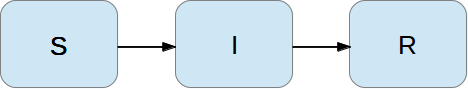
\includegraphics[width=0.7\linewidth]{fig/categories_SIR.png}}
\end{center}


Before we can compute with these, we must

\begin{itemize}
 \item know $\beta$ and $\nu$

 \item know $S(0)$ (many), $I(0)$ (few), $R(0)$ (0?)

 \item choose $\Delta t$
\end{itemize}

\noindent
\end{frame}

\begin{frame}[plain,fragile]
\frametitle{The computation involves just simple arithmetics}

\begin{itemize}
 \item Set $\Delta t=6$ minutes

 \item Set $\beta =0.0013$, $\nu =0.8333$

 \item Set $S(0)=50$, $I(1)$, $R(0)=0$
\end{itemize}

\noindent
\begin{align*}
S(\Delta t) &= S(0) - \Delta t\,\beta S(0)I(0)\approx 49.99\\
I(\Delta t) &= I(0) + \Delta t\,\beta S(0)I(0) -\Delta t\,\nu I(0)\approx 1.002\\
R(\Delta t) &= R(0) + \Delta t\,\nu R(0)\approx 0.0008333
\end{align*}

\begin{itemize}
 \item<2-> In reality, $S$, $I$, $R$ are integers and events are discrete (meet, get sick)

 \item<3-> In the model, we work with real numbers and continuous events

 \item<4-> Reasonable approximation in a not too small population
\end{itemize}

\noindent
\end{frame}

\begin{frame}[plain,fragile]
\frametitle{And we can continue...}

\begin{align*}
S(2\Delta t) &= S(\Delta t) - \Delta t\,\beta S(\Delta t)I(\Delta t)\approx 49.87\\
I(2\Delta t) &= I(\Delta t) + \Delta t\,\beta S(\Delta t)I(\Delta t) -\Delta t\,\nu I(\Delta t)\approx 1.011\\
R(2\Delta t) &= R(\Delta t) + \Delta t\,\nu R(\Delta t)\approx 0.00167
\end{align*}

Repeat...

\begin{align*}
S(3\Delta t) &= S(2\Delta t) - \Delta t\,\beta S(2\Delta t)I(2\Delta t)\approx 49.98\\
I(3\Delta t) &= I(2\Delta t) + \Delta t\,\beta S(2\Delta t)I(2\Delta t) -\Delta t\,\nu I(2\Delta t)\approx 1.017\\
R(3\Delta t) &= R(2\Delta t) + \Delta t\,\nu R(2\Delta t)\approx 0.0025
\end{align*}


\pause
\begin{block}{}
But this is getting boring! Let's ask a computer to do the work!
\end{block}
\end{frame}

\begin{frame}[plain,fragile]
\frametitle{First, some handy notation}

$S^n = S(n\Delta t)$,
$I^n = I(n\Delta t)$, $R^n = R(n\Delta t)$.

The equations can now be written as

\begin{align}
S^{n+1} &= S^n - \Delta t\,\beta S^nI^n
\label{SIR1:Sc}\\
I^{n+1} &= I^n + \Delta t\,\beta S^nI^n -\Delta t\,\nu I^n
\label{SIR1:Ic}\\
R^{n+1} &= R^n + \Delta t\,\nu R^n
\label{SIR1:Rc}
\end{align}
\end{frame}

\begin{frame}[plain,fragile]
\frametitle{We variables, arrays, and a loop we can program}

Suppose we want to compute until $t=N\Delta t$, i.e., for $n=0,1,\ldots,N-1$.
We can store $S^0, S^1, S^2, \ldots, S^N$ in an array (or list).

Python (Matlab):

\begin{minted}[fontsize=\fontsize{9pt}{9pt},linenos=false,mathescape,baselinestretch=1.0,fontfamily=tt,xleftmargin=7mm]{python}
t = linspace(0, N*dt, N+1)  # all time points
S = zeros(N+1)
I = zeros(N+1)
R = zeros(N+1)

for n in range(N):
    S[n+1] = S[n] - dt*beta*S[n]*I[n]
    I[n+1] = I[n] + dt*beta*S[n]*I[n] - dt*nu*I[n]
    R[n+1] = R[n] + dt*nu*I[n]
\end{minted}
\end{frame}

\begin{frame}[plain,fragile]
\frametitle{Here is the complete program}

Let time be measured in hours.

\begin{minted}[fontsize=\fontsize{9pt}{9pt},linenos=false,mathescape,baselinestretch=1.0,fontfamily=tt,xleftmargin=7mm]{python}
beta = 0.0013
nu =0.8333
dt = 0.1             # 6 min
D = 30               # simulate for D days
N = int(D*24/dt)     # corresponding no of hours

from numpy import zeros, linspace
t = linspace(0, N*dt, N+1)
S = zeros(N+1)
I = zeros(N+1)
R = zeros(N+1)

for n in range(N):
    S[n+1] = S[n] - dt*beta*S[n]*I[n]
    I[n+1] = I[n] + dt*beta*S[n]*I[n] - dt*nu*I[n]
    R[n+1] = R[n] + dt*nu*I[n]

# Plot the graphs
from matplotlib.pyplot import *
plot(t, S, 'k-', t, I, 'b-', t, R, 'r-')
legend(['S', 'I', 'R'], loc='lower right')
xlabel('hours')
show()
\end{minted}
\end{frame}

\begin{frame}[plain,fragile]
\frametitle{We have predicted a disease!}

\begin{center}  % inline figure
  \centerline{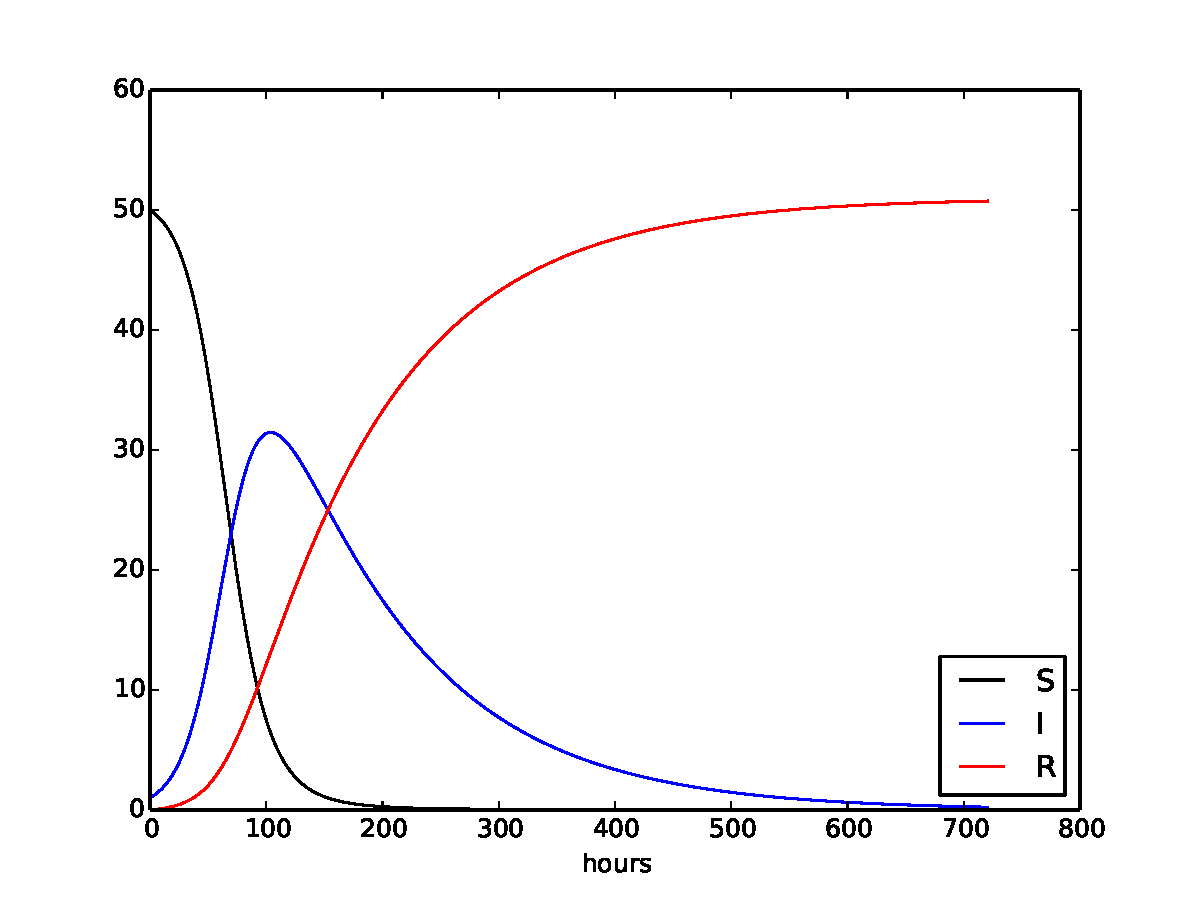
\includegraphics[width=0.9\linewidth]{fig/SIR1.pdf}}
\end{center}
\end{frame}

\begin{frame}[plain,fragile]
\frametitle{How much math and programming did we use?}

\begin{itemize}
 \item Plain arithmetics

 \item The concept of a graph (i.e., discrete function in time)

 \item Units

 \item Variable

 \item Array

 \item Loop

 \item Plotting
\end{itemize}

\noindent
\end{frame}

\begin{frame}[plain,fragile]
\frametitle{Detour: The standard mathematical approach}

We had from intuition established

\begin{align*}
S(t+\Delta t) &= S(t) - \Delta t\,\beta S(t)I(t)\\
I(t+\Delta t) &= I(t) + \Delta t\,\beta S(t)I(t) -\Delta t\,\nu I(t)\\
R(t+\Delta t) &= R(t) + \Delta t\,\nu R(t)
\end{align*}

The mathematician will now make a \emph{differential equations}. First,
divide by $\Delta t$ and move $S$, $I$, and $R$ to the left-hand side:

\begin{align*}
\frac{S(t+\Delta t) - S(t)}{\Delta t} &= - \beta S(t)I(t)\\
\frac{I(t+\Delta t) - I(t)}{\Delta t} &= \beta t S(t)I(t) -\nu I(t)\\
\frac{R(t+\Delta t) - R(t)}{\Delta t} &= \nu R(t)
\end{align*}
\end{frame}

\begin{frame}[plain,fragile]
\frametitle{A derivative arises as $\Delta t\rightarrow 0$}

In any calculus book, the derivative of $S$ at $t$ is defined as

\[ S'(t) = \lim_{t\rightarrow 0}\frac{S(t+\Delta t) - S(t)}{\Delta t}\]

If we let $\Delta t\rightarrow 0$, we get derivatives on the left-hand side:

\begin{align*}
S'(t) &= - \beta S(t)I(t)\\
I'(t) &= \beta t S(t)I(t) -\nu I(t)\\
R'(t) &= \nu R(t)
\end{align*}

This is a 3x3 system of differential equations for the functions
$S(t)$, $I(t)$, $R(t)$. For a unique solution, we need
$S(0)$, $I(0)$, $R(0)$.
\end{frame}

\begin{frame}[plain,fragile]
\frametitle{Bad news: we cannot solve these equations!}

\begin{block_mdfboxadmon}[Time to ask a numerical methods expert:]
Replace the derivative with a \emph{finite difference}, e.g.,

\[ S'(t) \approx \frac{S(t+\Delta t) - S(t)}{\Delta t}\]
which is accurate for small $\Delta t$.
\end{block_mdfboxadmon}



This brings us back to the first model, which we can solve
on a computer!
\end{frame}

\begin{frame}[plain,fragile]
\frametitle{Parameter estimation is needed for predictive modeling}

\begin{itemize}
 \item Any small $\Delta t$ will do

 \item One can reason about $\nu$ and say that $1/\nu$ is the mean
   recovery time for the disease (e.g., 1 week for a flu)

 \item $\beta$ must in some way be measured, but we don't know what it means...
\end{itemize}

\noindent

\begin{block_mdfboxadmon}[So what if we don't know $\beta$?]
\begin{itemize}
 \item Can still learn about the \emph{dynamics} of diseases

 \item Can find the sensitivity to and influence of $\beta$

 \item Can apply \emph{parameter estimation} procedures to fit $\beta$ to data
\end{itemize}

\noindent
\end{block_mdfboxadmon}
\end{frame}

\begin{frame}[plain,fragile]
\frametitle{Let us extend the model: no life-long immunity}

\begin{block_mdfboxadmon}[Assumption.]
After some time, people in the R category lose the immunity.
In a small time $\Delta t$ this gives a leakage $\Delta t\,\gamma R$
to the S category. ($1/\gamma$ is the mean time for immunity.)
\end{block_mdfboxadmon}




\begin{center}  % inline figure
  \centerline{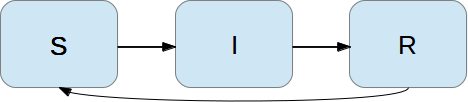
\includegraphics[width=0.7\linewidth]{fig/categories_SIR_feedback.png}}
\end{center}


\begin{align}
S^{n+1} &= S^n - \Delta t\,\beta S^nI^n + \color{red}{\Delta t\,\gamma R^n}
\label{SIR2:S}\\
I^{n+1} &= I^n + \Delta t\,\beta S^nI^n -\Delta t\,\nu I^n
\label{SIR2:I}\\
R^{n+1} &= R^n + \Delta t\,\nu R^n - \color{red}{\Delta t\,\gamma R^n}
\label{SIR2:R}
\end{align}

No complications in the computational model!
\end{frame}

\begin{frame}[plain,fragile]
\frametitle{The effect of loss of immunity}

$1/\gamma = 50$ days. $\beta$ reduced by 2 and 4:


\begin{center}  % inline figure
  \centerline{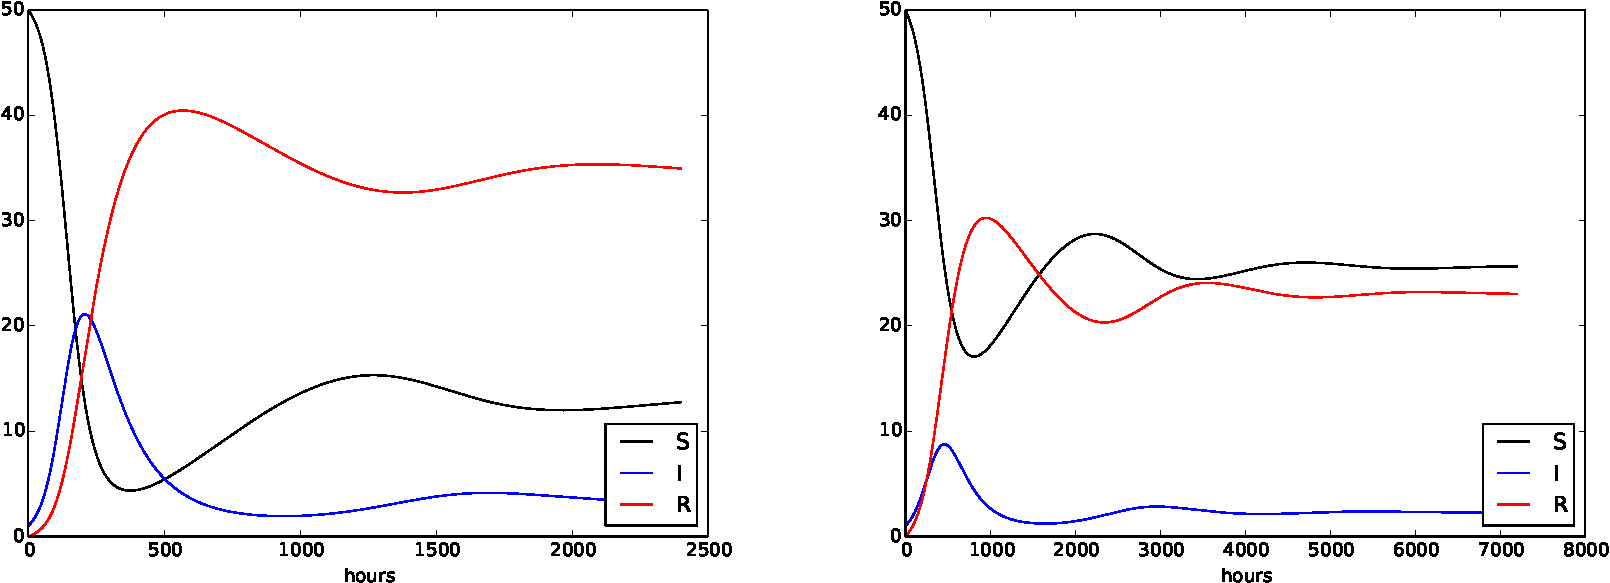
\includegraphics[width=0.9\linewidth]{fig/SIR2.pdf}}
\end{center}
\end{frame}

\begin{frame}[plain,fragile]
\frametitle{What is the effect of vaccination?}

\begin{block_mdfboxadmon}[Assumptions.]
A fraction $p$ of the S category, per time unit, is vaccinated with
success. Then in time $\Delta t$, $p\Delta t S$ will move to a
vaccinated category, V. This does not affect the I and R categories.
\end{block_mdfboxadmon}




\begin{center}  % inline figure
  \centerline{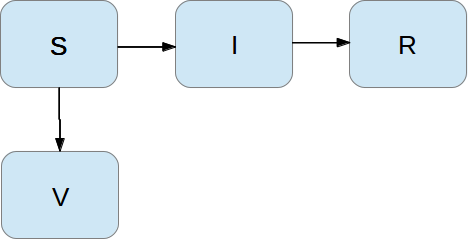
\includegraphics[width=0.4\linewidth]{fig/categories_SIRV.png}}
\end{center}


\begin{align}
S^{n+1} &= S^n - \Delta t\,\beta S^nI^n + \Delta t\,\gamma R^n - \color{red}{p\Delta t S^n}
\label{SIR3:S}\\
V^{n+1} &= V^n + \color{red}{p\Delta t S^n}
\label{SIR3:V}\\
I^{n+1} &= I^n + \Delta t\,\beta S^nI^n -\Delta t\,\nu I^n
\label{SIR3:I}\\
R^{n+1} &= R^n + \Delta t\,\nu R^n - \Delta t\,\gamma R^n
\label{SIR3:R}
\end{align}

Implementation: Just add array for $V^n$ and add equation.
\end{frame}

\begin{frame}[plain,fragile]
\frametitle{Many possibilities for adjusting the model...}

The effect of vaccination decreases, so we may move people back to
the S category (term proportional to $\Delta t V$).


\begin{center}  % inline figure
  \centerline{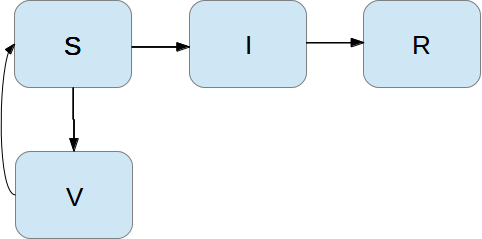
\includegraphics[width=0.7\linewidth]{fig/categories_SIRV_feedback.png}}
\end{center}
\end{frame}

\begin{frame}[plain,fragile]
\frametitle{Effect of adding vaccination}

\begin{center}  % inline figure
  \centerline{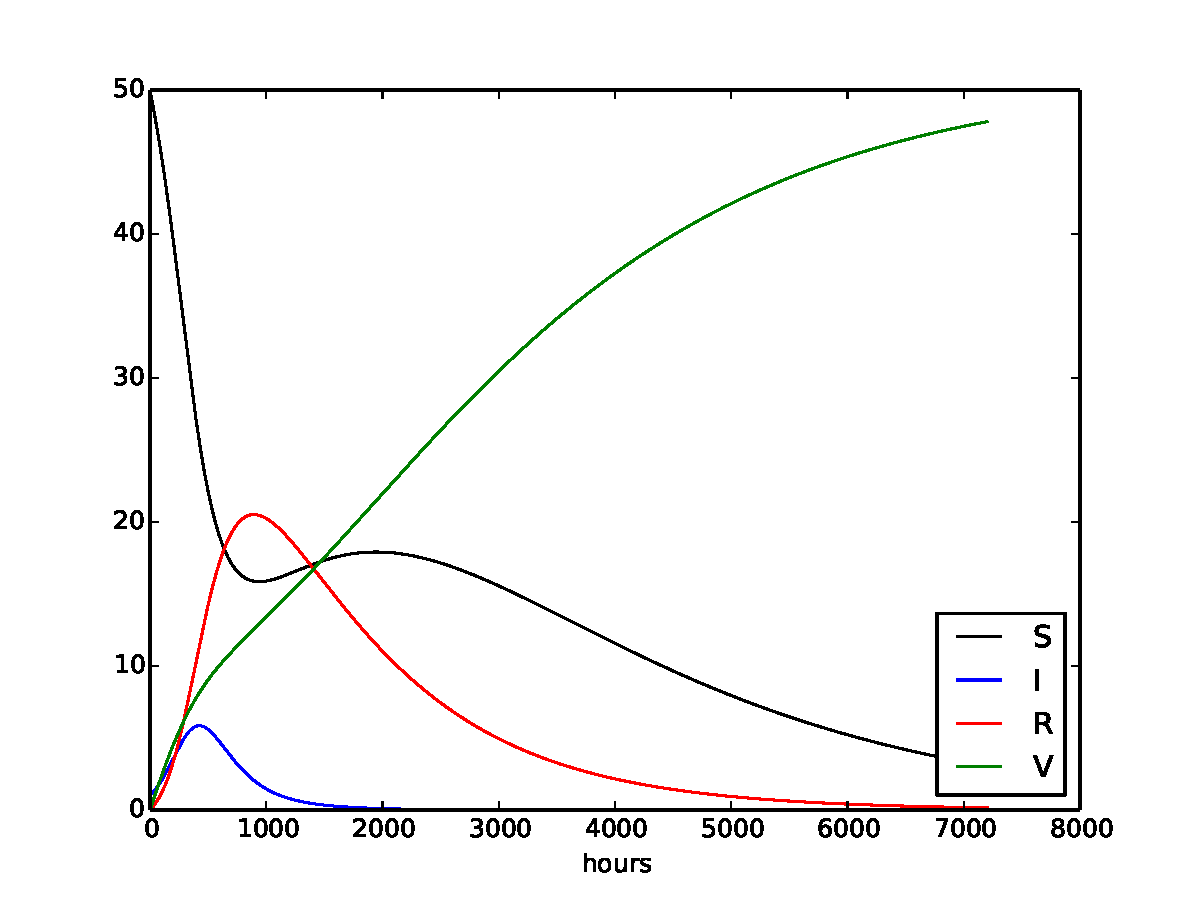
\includegraphics[width=0.8\linewidth]{fig/SIRV1.pdf}}
\end{center}


($p=0.005$)
\end{frame}

\begin{frame}[plain,fragile]
\frametitle{What is the effect of an intensive vaccination campaign?}

10 times more intense vaccination for 10 days, 6 days after outbreak:

\begin{equation*} p(t) = \left\lbrace\begin{array}{ll}
0.05,& 6\leq t\leq 15,\\
0,& \hbox{otherwise} \end{array}\right.\end{equation*}

Implementation: Let $p^n$ be an array as $V^n$. Set $p^n=0.05$ for
$n=6\cdot 24/0.1,\ldots, 15\cdot 24/0.1$ ($\mbox{days}\cdot 24 \mbox{h per
day}\Delta t$).
\end{frame}

\begin{frame}[plain,fragile]
\frametitle{Effect of vaccination campaign}

\begin{center}  % inline figure
  \centerline{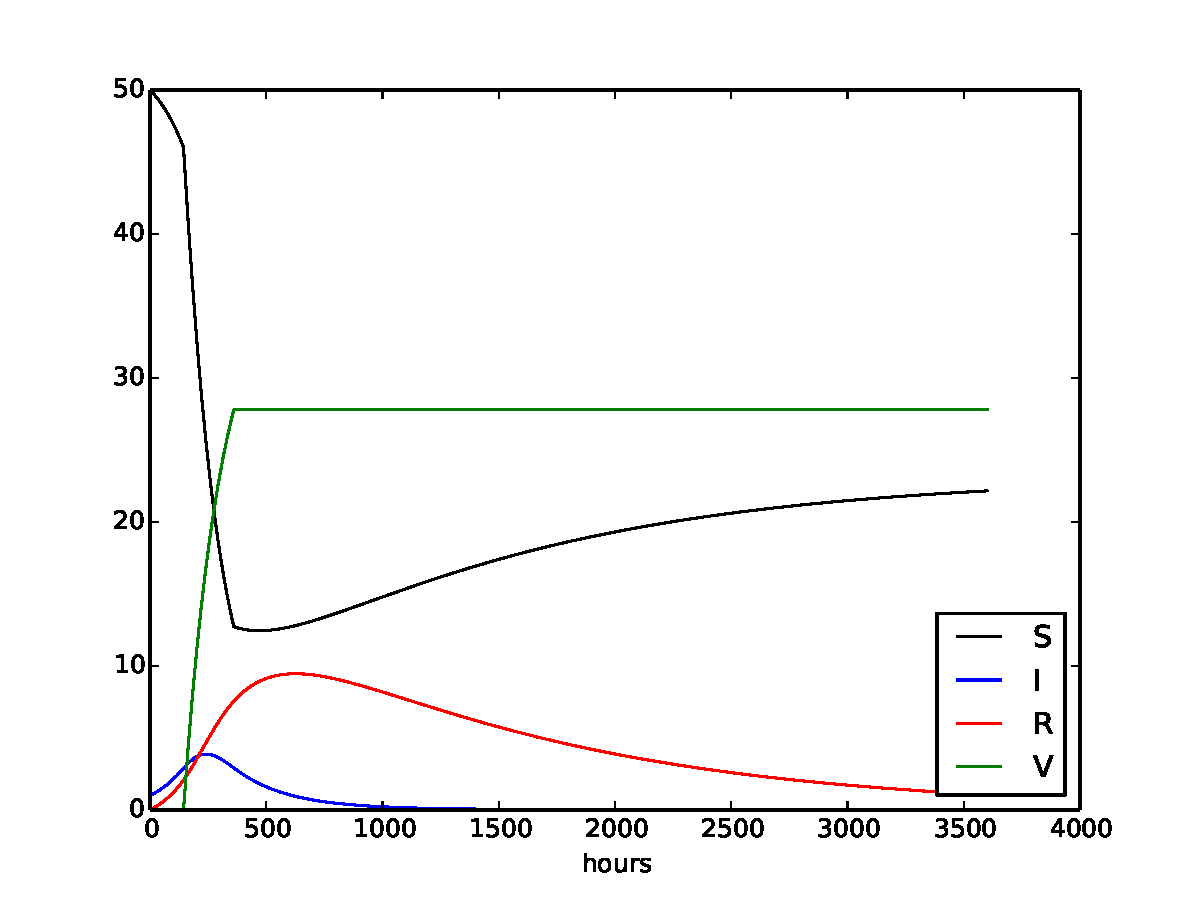
\includegraphics[width=0.8\linewidth]{fig/SIRV2.pdf}}
\end{center}


Could now let the computer run a lot of cases and find the optimal
vaccination period.
\end{frame}

\begin{frame}[plain,fragile]
\frametitle{We can experiment with other campaigns}

\begin{columns}
\column{0.3\textwidth}
\begin{center}  % inline figure
  \centerline{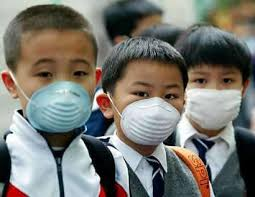
\includegraphics[width=0.9\linewidth]{fig/disease2.jpg}}
\end{center}


\column{0.7\textwidth}
Masks lower $\beta$:

\begin{equation*} \beta(t) = \left\lbrace\begin{array}{ll}
\beta_1,& 0\leq t < 5,\\
\beta_2 < \beta_1,& t \geq 5\end{array}\right.
\end{equation*}

Very easy to implement. (Used to be complicated in differential
equation models...)

\end{columns}
\end{frame}

\begin{frame}[plain,fragile]
\frametitle{And now for something similar: zombification}

\begin{center}  % inline figure
  \centerline{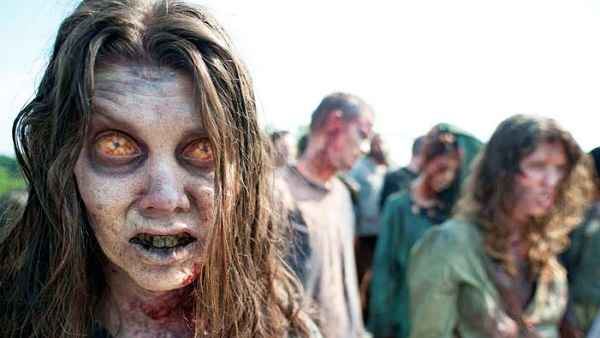
\includegraphics[width=0.9\linewidth]{fig/zombie1.jpg}}
\end{center}


\textbf{Zombification}: The disease that turns you into a zombie.
\end{frame}

\begin{frame}[plain,fragile]
\frametitle{Zombie modeling is almost the same as SIR modeling}

\begin{block_mdfboxadmon}[Categories.]
\begin{enumerate}
 \item S: susceptible humans who can become zombies

 \item I: infected humans, being bitten by zombies

 \item Z: zombies

 \item R: removed individuals, either conquered zombies or dead humans
\end{enumerate}

\noindent
\end{block_mdfboxadmon}



Mathematical quantities: $S(t)$, $I(t)$, $Z(t)$, $R(t)$

Zombie movie: \emph{The Night of the Living Dead}, Geoerge A. Romero, 1968
\end{frame}

\begin{frame}[plain,fragile]
\frametitle{Dynamics of the zombie SIZR model}

\begin{center}  % inline figure
  \centerline{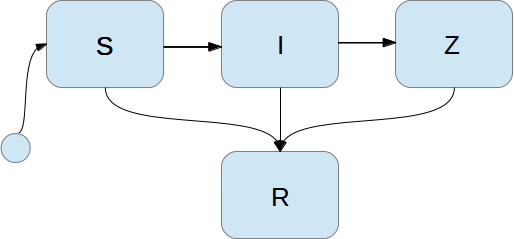
\includegraphics[width=0.4\linewidth]{fig/categories_SIZR.png}}
\end{center}


\begin{enumerate}
 \item<2-> Susceptibles are infected by zombies: $-\Delta t\beta SZ$ in time $\Delta t$ (cf.~the $\Delta t\,\beta SI$ term in the SIR model).

 \item<3-> Susceptibles die naturally or get killed and then enter the removed category. The no of deaths in time $\Delta t$ is $\Delta t\delta_S S$.

 \item<4-> We also allow new humans to enter the area with zombies (necessary in a war on zombies): $\Delta t\Sigma$ during a time $\Delta t$.

 \item<5-> Some infected turn into zombies (Z): $\Delta t\rho I$, while others die (R): $\delta_I\Delta t I$.

 \item<6-> Nobody from R can turn into Z (important - otherwise zombies win).

 \item<7-> Killed zombies go to R: $\Delta t\alpha SZ$.
\end{enumerate}

\noindent
\end{frame}

\begin{frame}[plain,fragile]
\frametitle{The four equations in the SIZR model for zombification}

\begin{align*}
S^{n+1} &= S^n + \Delta t\,\Sigma - \Delta t\,\beta S^nZ - \Delta t\,\delta_S S^n\\
I^{n+1} &= I^n + \Delta t\,\beta S^nZ^n - \Delta t\,\rho I^n - \Delta t\,\delta_I I^n\\
Z^{n+1} &= Z^n + \Delta t\,\rho I^n - \Delta t\,\alpha S^nZ^n\\
R^{n+1} &= R^n + \Delta t\,\delta_S S^n  + \Delta t\,\delta_I I^n +
\Delta t\,\alpha S^nZ^n
\end{align*}


\begin{block_mdfboxadmon}[Interpretation of parameters:]
\vspace{0.5mm}\par\noindent
{\footnotesize 
\begin{itemize}
  \item $\Sigma$: no of new humans brought into the zombified area per unit time.

  \item $\beta$: the probability that a theoretically possible human-zombie pair actually meets physically, during a unit time interval, with the result that the human is infected.

  \item $\delta_S$: the probability that a susceptible human is killed or dies, in a unit time interval.

  \item $\delta_I$: the probability that an infected human is killed or dies, in a unit time interval.

  \item $\rho$: the probability that an infected human is turned into a zombie, during a unit time interval.

  \item $\alpha$: the probability that, during a unit time interval, a theoretically possible human-zombie pair fights and the human kills the zombie.
\end{itemize}

\noindent
\par}
\end{block_mdfboxadmon}
\end{frame}

\begin{frame}[plain,fragile]
\frametitle{Simulate a zombie movie!}

\begin{columns}
\column{0.5\textwidth}
\begin{block_mdfboxadmon}[Three fundamental phases.]
\begin{enumerate}
\item The initial phase (4 h)

\item The hysteric phase (24 h)

\item The counter attack phase (5 h)
\end{enumerate}

\noindent
\end{block_mdfboxadmon}



\column{0.5\textwidth}
\begin{center}  % inline figure
  \centerline{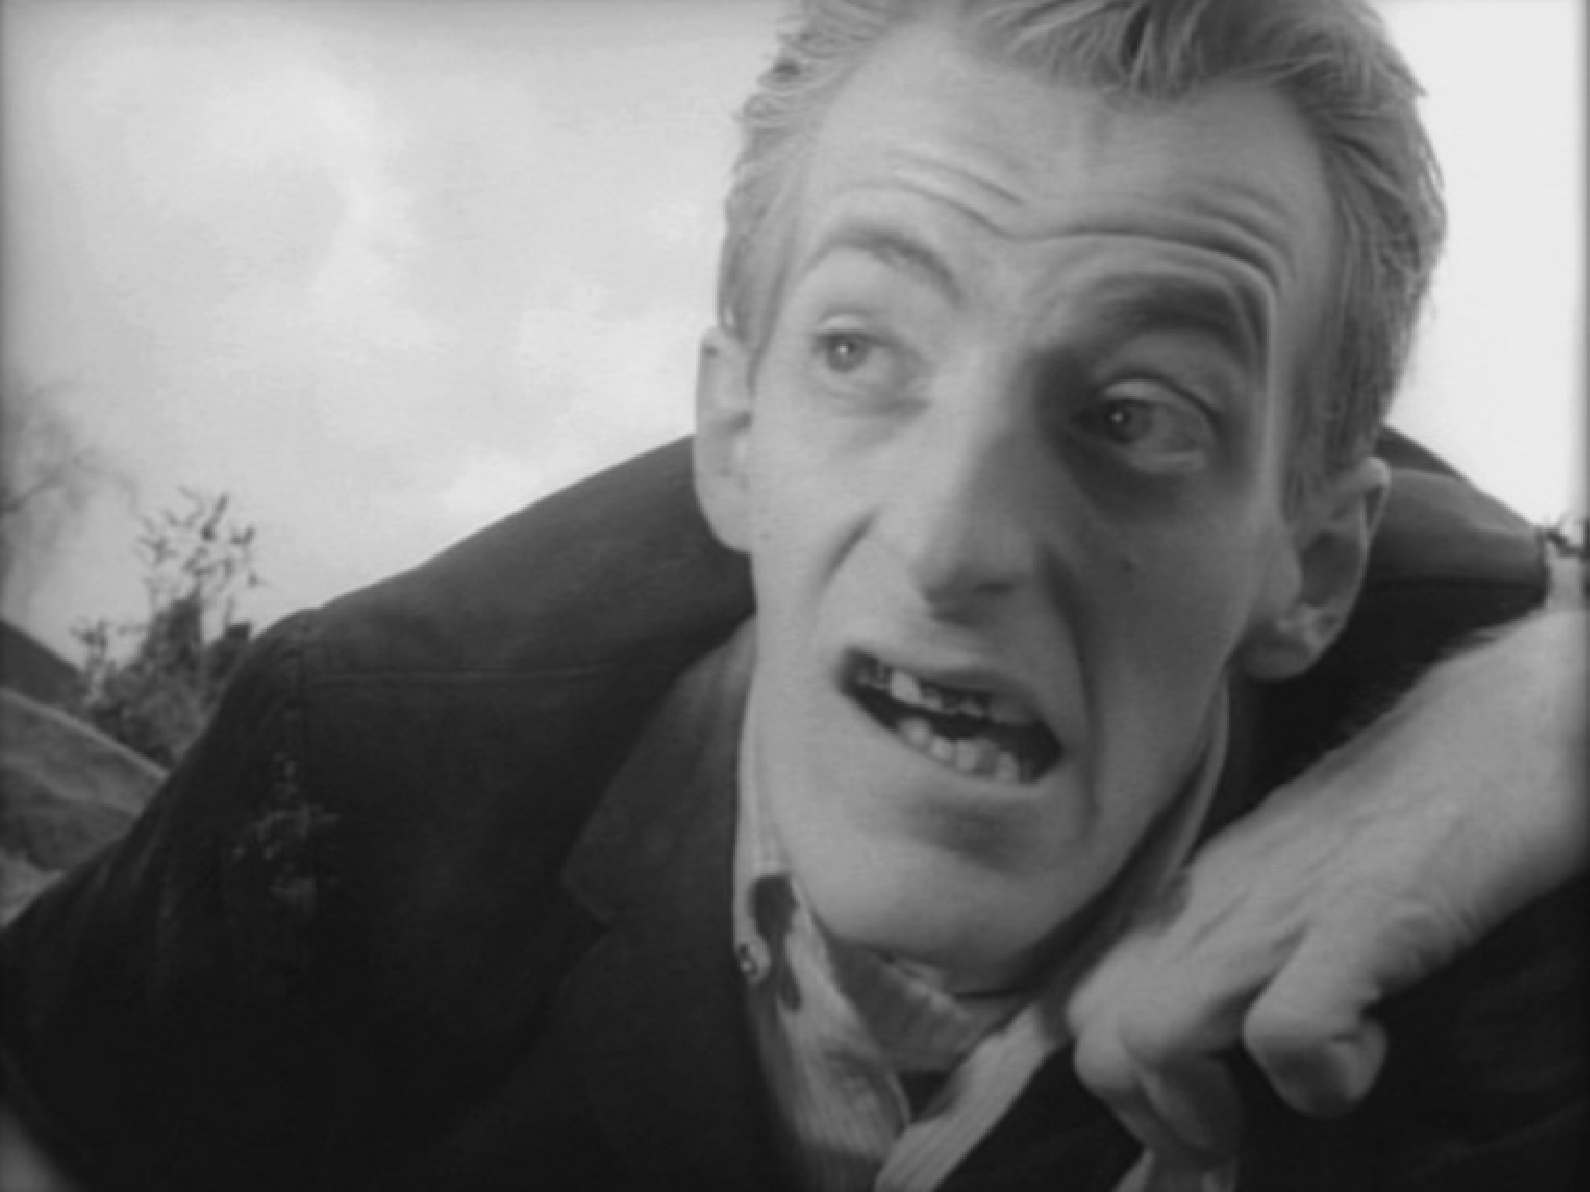
\includegraphics[width=0.9\linewidth]{fig/TNotLD.pdf}}
\end{center}


\end{columns}






\pause
\begin{block}{}
How do we do this? As $p$ in the vaccination campaign - the parameters
take on different constant values in different time intervals.
\end{block}



\pause
\begin{block}{}
H. P. Langtangen and K.-A. Mardal and P. Røtnes:
Escaping the Zombie Threat by Mathematics, in
A. Whelan et al.: \emph{Zombies in the Academy - Living Death in Higher Education},
University of Chicago Press, 2013
\end{block}
\end{frame}

\begin{frame}[plain,fragile]
\frametitle{Effective war on zombies}

Introduce attacks on zombies at selected times $T_0, T_1, \ldots, T_m$.

Model: Replace $\alpha$ by

\[ \alpha_0 + \omega (t),\]
where $\alpha_0$ is constant and $\omega(t)$ is a series of
Gaussian functions (peaks) in time:

\[ \omega(t) = a\sum_{i=0}^m \exp{\left(-\frac{1}{2}\left({t - T_i\over\sigma}\right)\right)}
\]

Must experiment with values of $a$ (strength), $\sigma$ (duration is $6\sigma$),
point of attacks ($T_i$)
\end{frame}

\begin{frame}[plain,fragile]
\frametitle{Summary}

\begin{itemize}
 \item A complex spreading is diseases can be modeled by intuitive, simple
   accounting of movement between categories

 \item Such models are knowns as \emph{compartment models}

 \item Result: difference equations that are easy to simulate on a computer

 \item (Can let $\Delta t\rightarrow 0$ and get differential equations)

 \item Easy to add new effects (vaccination, campaigns, zombification)
\end{itemize}

\noindent
\end{frame}

\end{document}
